\chapter{Introduction}\label{ch:Intro}
\section{Challenge, Motivation and Our Approach}
\par The remarkable success of cellular wireless communication technologies make it possible for smartphones to be widely used, which generates dramatical demand increase for mobile broadband capacity every year. \reminder{Add reference} As a result, the conventional cellular bands below 3 GHz are very crowded. With the severe shortage in conventional cellular bands, millimeter wave (mmWave) \reminder{30G and above?} frequency spectrum has been considered as a key component to address the bandwidth deficiency in the next generation wireless communication network.  \reminder{Add reference, also added some words describing the recent advances in hardware and systems of mmWave}
\subsection{Next Generation Cellular Network}
\par There are fundamental differences between current cellular communication system and mmWave communication system, in terms of high propagation loss, low delay and sensitivity to blockage. \reminder{high loss and blockage is related to mmWave, low delay is driving by applications, you can say mmWave system make it more challening} These characteristics of mmWave channel result in tough challenges to fully exploit its potential. Fading can substantially affect the performance of a wireless communication system. In general, fading can be divided into two categories: large-scale fading and small-scale fading. Small-scale fading is caused by multipath propagation. Large-scale fading, which is also known as shadow fading, is caused by obstacles in the propagation path. Electromagnetic waves have weak ability to diffract around obstacles with a size significantly larger than its wavelength. High frequency mmWave has small wavelength, which makes it more sensitive to blockage caused by small size obstacles like buildings, trees and even nearby pedestrians or vehicles. Therefore, shadow fading has significant impact on the performance of the next generation wireless communication system. Shadow fading can cause significant received power loss. We can conclude from what we have stated above that mmWave channel can be severely vulnerable to shadowing resulting in outages, rapidly changing channel conditions and intermittent connectivity. \reminder{I suggest you remove small scale fading, which might not be a problem at all since most mmWave system will be lucky to get even one path; WHen you talk about shadowing, talking from the point that those shadow are different from lower band, which caused mostly by buildings. In mmWave system, small object can cause shadowing, thus the character would be different}

\reminder{before you jump to a detailed shadow model, expand the discussion above by adding due to the low delay required by applications, even though mmWave have very high bandwidth, it shortcoming has to be mitigated. One way to do so is to use multiple BS to provide diversity, and that's why you care about correlated shadow fading. You should also talk about the on-off nature of mmWave links, and why that will affect transport layer, which is why you take TCP as part of your thesis study.}
\par Shadow fading is an important factor to be considered when analyzing the system performance. In most cases, shadow fading is assumed to be temporally and spatially independent to simplify the analysis of the system performance. Obviously this is not the real scenario, especially for next generation wireless communication network. For mmWave communication networks, the cell size will become mush smaller than current LTE cell size due to high propagation loss~\reminder{add citation}. When cell size becomes comparable with the size of obstacles that cause shadow fading, shadow fading cannot be considered as spatially independent. Due to the aforementioned characteristics of mmWave channel and next generation wireless communication network, this thesis focuses on investigating the system performance under correlated shadow fading. Since there is no consensus on standard mmWave channel, we study the system performance under correlated shadow fading of the legacy cellular spectrum frequency and suggest it can be applied to mmWave channel in the future. 

\reminder{the following should belongs to your chapter, not introduction}
\par At first, we choose distance-angle correlation model\reminder{cite} for shadow fading and investigate the correlated shadow fading problem in a single-cell cellular network. We find that correlated shadow fading could lead to correlated outage and long outage durations. \reminder{With non-correlated shadow model, we can only analysis a snapshot of the system. However, in order to predict application performance over time, such as outage durations, correlated shadow fading model is necessary}. To mitigate shadow fading and decrease shadow durations, wireless relays are deployed. The performance of three different relay deployments with different relay densities are investigated. Theoretical analysis and simulations of outage performance are compared between different relay placement scenarios. \cite{The following sentence seems from your paper,  you should change it since this is the intro of dissertation}This work illustrate that uniformly spaced relays perform better than the randomly spaced. Single-cell model is not suitable for analyzing next generation wireless communication networks. Therefore, extending the investigation to multi-cell network is necessary. \reminder{why single cell analysis is not suitable? Is it because you believe the future network cannot rely on a single BS since diversity is essential? Explain}The disadvantage of the distance-angle correlation model is that it scales with cell size when considering denser network. This is not realistic since the obstacle size will not scale with the cell size. \reminder{Don't understand why scale is a bad thing. Are you trying to say the network is denser so cell radius is small? If so, why the distance angle cannot be used? Purely because of complexity}Due to this feature, we choose to use exponential correlation model when we study multi-cell network. 

\par Exponential correlation model\reminder{cite} has been widely used by researchers. Considering a single-cell model, exponentially correlated shadow fading can be modeled as a first-order autoregressive process. \reminder{Should add more background before talking details, I still feel such detail should not be in intro section} Given this feature, a first-order Markov chain model is developed and validated. The Markov chain model is constructed by partitioning the entire shadow fading range into a finite number of intervals. The state transition matrix of the Markov chain is derived from the joint probability distribution of correlated log-normal shadow fading. Based on the proposed Markov chain model, the frequency and duration of outage near the edge of a single cell can be analyzed. To validate the Markov chain model, correlated Gaussian random fields are simulated to analyze the outage frequency and durations due to correlated shadow fading. Comparing the simulation results with the Markov chain model results, we conclude \reminder{Don't show your results, intro should be a place to tell people why the things you are going to talk about is important, and how you plan to do it, instead of results.} that the proposed Markov chain model is an efficient way to describe the channel variations, and the user experienced outage behavior of the channel. This Markov chain model can not be extended to multi-cell system because of the existing of interference from other base stations (BSs). \reminder{Don't understand previous sentence} To further investigate the performance of multi-cell system, we run simulation for different BS densities. Two scenarios are investigated: MU connecting to the nearest BS and MU connecting to the BS with strongest signal. We calculate signal-to-noise-and-interference ratio (SINR) for the mobile user (MU) with regard to different scenarios. Outage probability and outage duration can be generated from the SINR result. We conclude \reminder{no "conclude"} that increasing BS densities can decrease outage probability when MU is connected to the nearest BS. Outage duration will decrease when increasing the BS density in both cases. 

\par \reminder{Before talking about simulation. Explain why you care about higher layer performance, why TCP will have problem on mmWave channels} In order to investigate application performance, an NS-2 \reminder{?} based link layer model is employed. The simulation model is based on an Ethernet channel with high capacity and low delay. We extended the model to allow the physical link to be periodic on-off to mimic the mmWave channel. Existing TCP congestion control protocols are tested on this channel. Both throughputs and the variation of congestion windows are showed with regard to different channel behaviors. A data-driven fast congestion prediction algorithm is proposed based on the idea of Explicit Congestion Notification (ECN). This fast congestion prediction algorithm can be utilized to design next generation transport layer protocols.
\subsection{Correlated Shadow Fading Models}
\par In most cases, shadow fading is modeled as an independent log-normal distribution \cite{goldsmith2005wireless} with a standard deviation derived from empirical measurements. An independent log-normal shadowing model is used widely when shadow fading cannot be ignored. But this model fails to capture the spatial correlations in shadow fading, which has been proved to be not negligible in \cite{graziano1978propagation}, \cite{marsan1990shadowing} and \cite{liberti1992statistics}. In \cite{szyszkowicz2010feasibility}, the author elaborated several models for correlated shadow fading,  investigated their feasibility and presented the physical plausibility of each model. Correlations can be divided into two categories: autocorrelation and cross-correlation as in Figure \ref{correlation}. Autocorrelation is the correlation between two receivers receiving signal from the same transmitting node. Cross-correlation considers two transmitting nodes transmitted to the same receiver. Autocorrelation and cross-correlation are symmetric in mathematical sense and can be investigated in the same manner.
\begin{figure} 
\centering
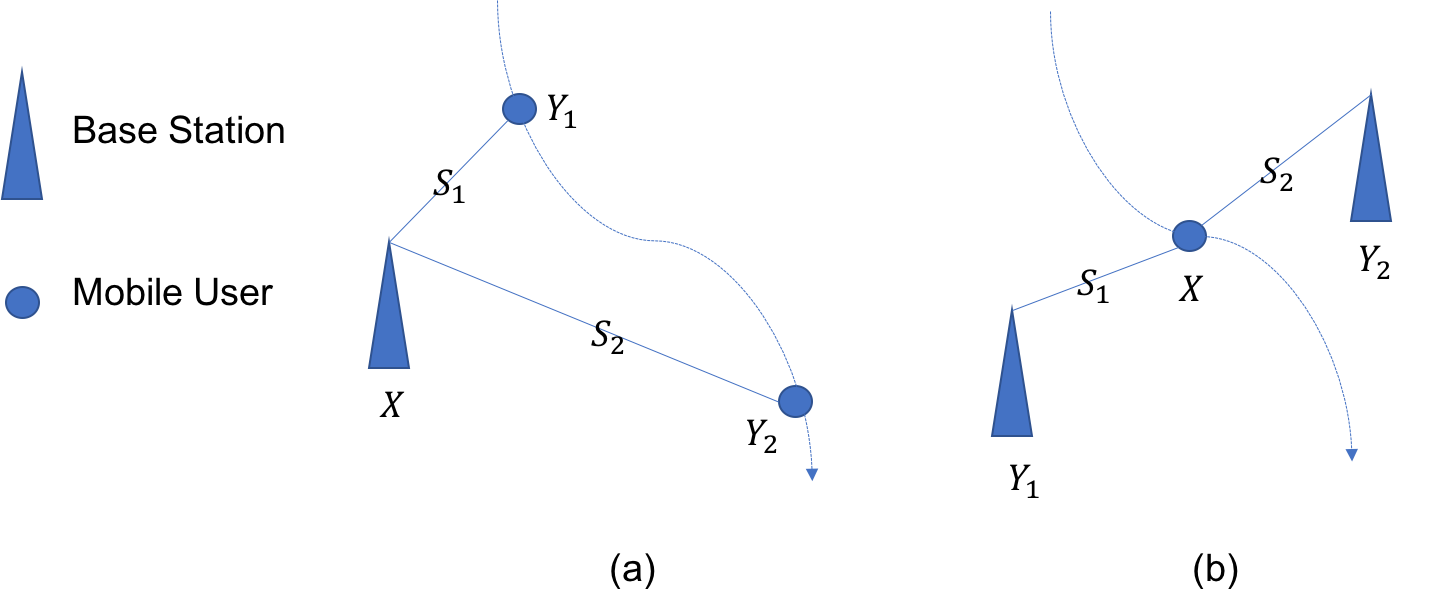
\includegraphics[width=14cm]{correlation.png}
\caption{(a) Shadowing autocorrelation for a mobile user, (b) Shadowing cross-correlation for a mobile user}
\label{correlation}
\end{figure}
\par Autocorrelation and cross-correlation models can be described as in Figure \ref{geometry}. There are $N$ points $Y_{1}, \cdots, Y_{N}$.  $S_{i}$ is the logarithm of the power attenuation due to shadowing on each path $\vec{r_{i}}$. $\mathbb{E}\{S_{i}\} = 0$ since shadow fading has correlated log-normal distribution. The log-variance of shadow fading can be characterized as 
\begin{equation}
\sigma_{i}^{2} = \mathbb{VAR}\{S_{i}\} = \sigma_{S}^2(\vec{r_{i}})
\label{sigma}
\end{equation}
\begin{figure} 
\centering
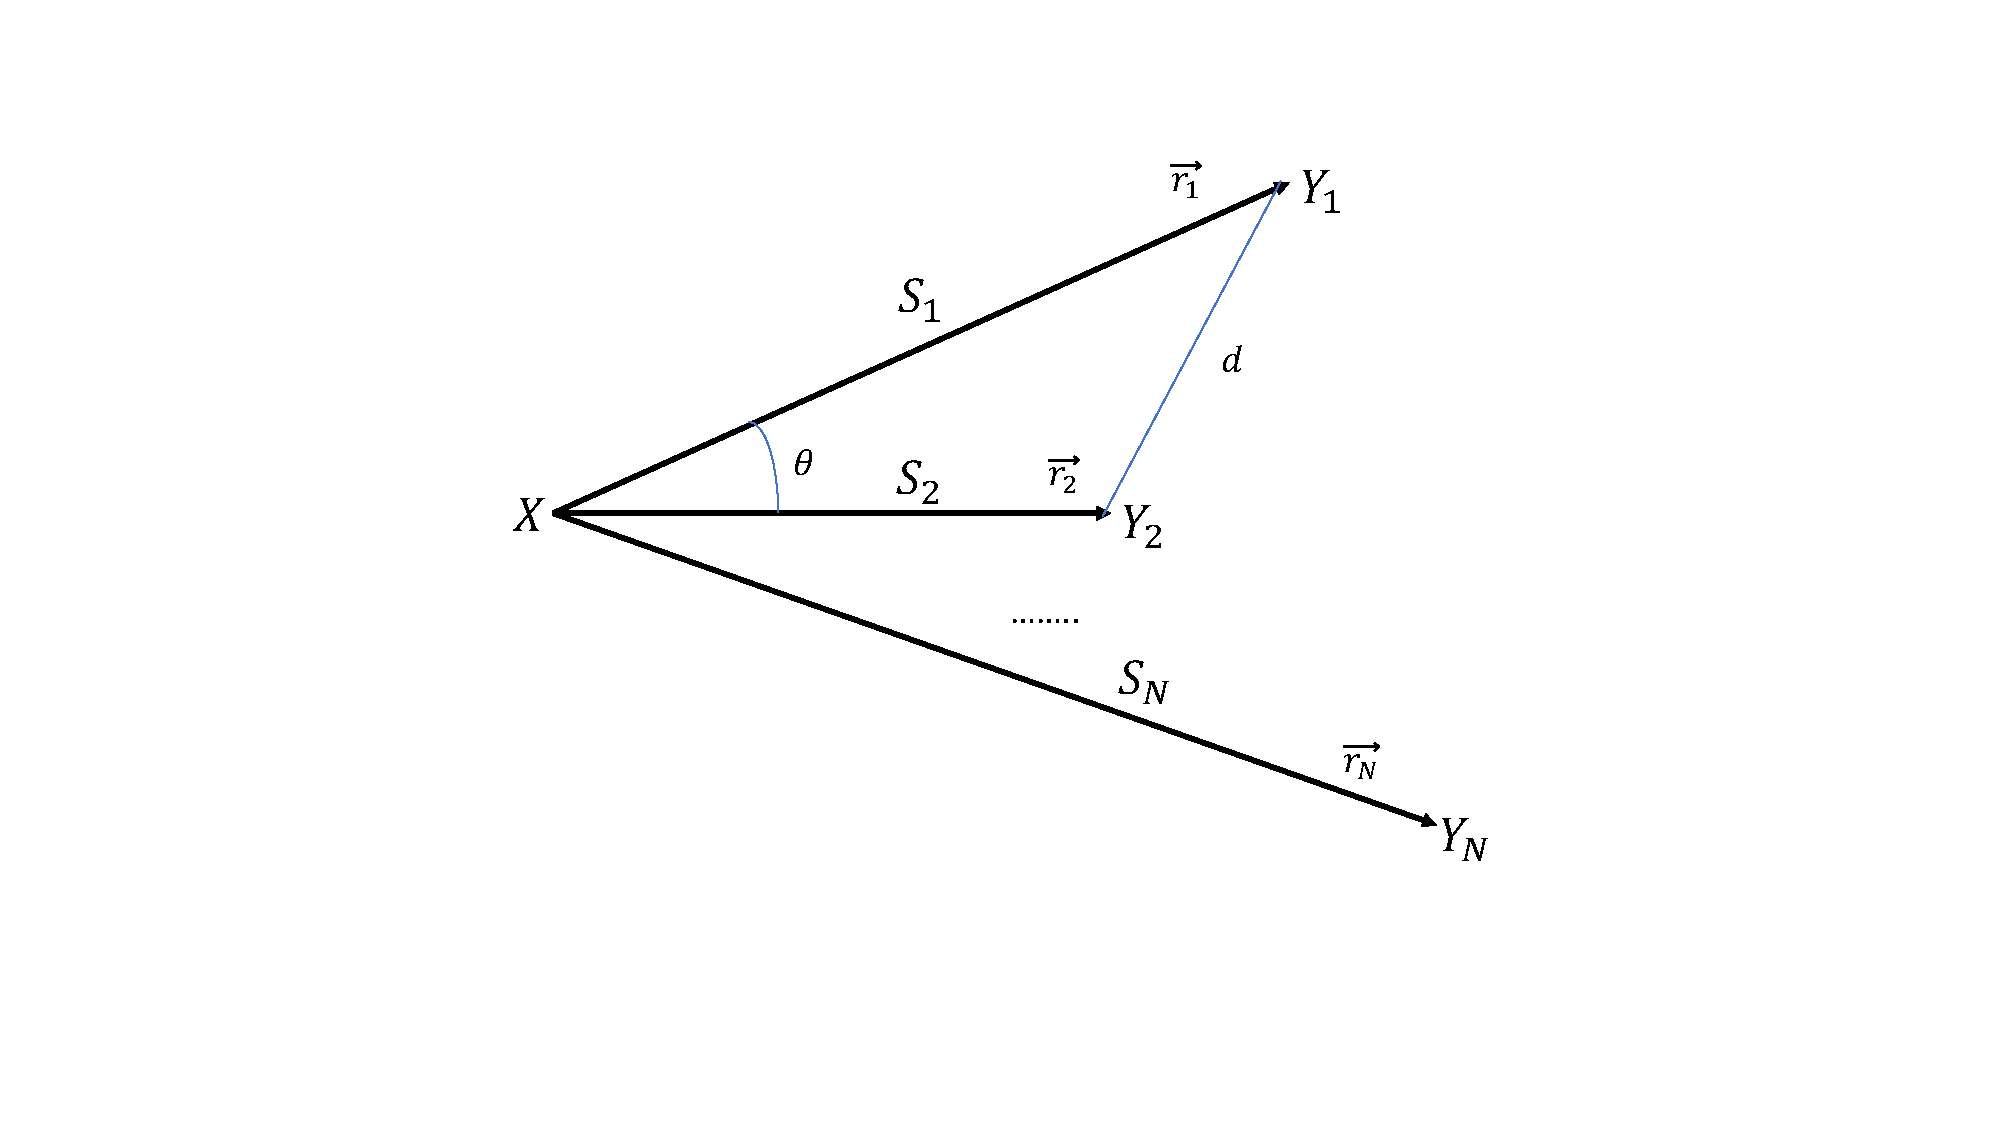
\includegraphics[width=14cm]{FadingGeometry.pdf}
\caption{Generic geometry of shadowing autocorrelation and cross-correlation}
\label{geometry}
\end{figure}
This variance is considered as constant after a certain distance \cite{kitchener2006correlated}.
\par The correlation coefficients can be defined as
\begin{equation}
\begin{split}
& \rho_{i,j} = \mathbb{E}\{S_{i}S_{j}\}/\sigma_{i}\sigma_{j} = h(\vec{r_{i}}, \vec{r_{j}}), i \neq j \\
& \rho_{i,i} = 1.
\end{split}
\end{equation}
The following properties will be held:
\begin{itemize} 
\item $-1\leq h(\vec{r_{i}}, \vec{r_{j}}) \leq 1$
\item $h(\vec{r_{i}}, \vec{r_{j}})  = h(\vec{r_{j}}, \vec{r_{i}}) $
\end{itemize}
The correlation matrix of $\mathbf{S} = [S_{1}, \cdots, S_{N}]$ is:
\begin{equation}
\mathbf{K} = \left[\begin{array}{cccc}
\sigma_{1}^{2} & \sigma_{1}\sigma_{2}\rho_{1,2} & \cdots & \sigma_{1}\sigma_{N}\rho_{1,N}\\
\sigma_{1}\sigma_{2}\rho_{1,2} & \sigma_{2}^{2} & \cdots & \sigma_{2}\sigma_{N}\rho_{2,N}\\
\vdots & \ddots & \ddots & \vdots\\
\sigma_{1}\sigma_{N}\rho_{1,N} & \sigma_{2}\sigma_{N}\rho_{2,N} & \cdots & 1\\
\end{array}\right].
\end{equation}
For $\mathbf{K}$ to be a valid covariance matrix, it is necessary that $\mathbf{K}$ is positive semidefinite(\emph{psd}).
\par By grouping the measurements along one variable in several ways, $h$ can be expressed as a function of a single variable in the following three forms:
\begin{itemize}
\item absolute distance (between $Y_{1}$ and $Y_{2}$): $d = \Vert \vec{r_{1}}- \vec{r_{2}}\Vert$ .
\item angle of arrival separation: $\theta = \vert\angle\vec{r_{1}}-\angle\vec{r_{2}}\vert\in [0^\circ, 180^\circ]$ 
\item arrival distance ratio (in decibels): $R=\vert10\log_{10}r_{1}/r_{2}\vert=(10/\ln 10)\vert \ln r_{1}-\ln r_{2}\vert$
\end{itemize}
A correlation model needs to satisfy as many as the following criteria to become a precise model:
\begin{itemize}
\item $h(\vec{r_{i}}, \vec{r_{j}}) \approx 1$ for $\vec{r_{i}}\approx \vec{r_{j}}$.
\item $h(\vec{r_{i}}, \vec{r_{j}}) \ll 1$ for $\Vert \vec{r_{i}}- \vec{r_{j}}\Vert\gg0$.
\item $h$ should be a nonincreasing function in $\theta$, $R$ and $d$.
\item $h$ should be nonnegative.
\item $h$ should be small for large $\theta$ and approach zero for $\theta\approx180^\circ$, and $r_{1}$ and $r_{2}$ large.
\item Continuity: a small change in $\vec{r_{i}}$ should result in small change in $h(\vec{r_{i}}, \vec{r_{j}})$.
\item Correlation should not depend on $d$ only.
\end{itemize}
Considering the above criteria, the author of \cite{szyszkowicz2010feasibility} recommended a correlated shadow fading model with distance and angle in \cite{szyszkowicz2011interference}, and provided a fast simulation method to generate the correlated shadowing field. We use this model to analyze single-cell system performance and discuss how cooperative communication can help to mitigate shadow fading. 

\par After investigating the single cell system, we further analyzed multi-cell system performance. The aforementioned distance-angle model cannot be applied to this scenario. The correlation coefficient is a piecewise linear function of $\theta$ and $R$. \reminder{Refer to the equation of the model} When the cell size scales, $\theta$ and $R$ remain the same, which means the correlation between two different positions also scales. Since the size of obstacles which generate shadow fading does not change with cell size, this model violate the physical characteristics of shadow fading. Exponentially correlated shadow fading is the most widely used model. To investigate the multi-cell system performance with correlated shadow fading, we choose the exponential correlation model. Exponential correlation model can be modeled as a Markov chain model in the single-cell case. This Markov model can be used to simplify the analysis of system performance. However, this Markov model cannot be used to analyze the performance of multi-cell system due to the existing of interference. Simulations are run to study the outage probability and outage duration of the multi-cell system given different network topologies. 


\subsection{Transmission Control Protocol (TCP)}
\par TCP is the transport layer protocol that provides reliable connection-oriented and in-order delivery service to applications \cite{panwar2004tcp}. TCP uses error control, flow control and congestion control to achieve this. When incoming traffic demand to the network exceeds its capacity, congestion happens and propagates to other connected networks. Congestions in network can generate long delay and high packet loss rate. Due to fading, mmWave cellular network might be unstable and switching between Line-Of-Sight (LOS) and Non-Line-Of-Sight (NLOS) states frequently, which results in large variations in data rate. This behavior determines that mmWave cellular network is prone to congestion. Therefore, design an efficient congestion control protocol is necessary for next generation wireless communication network. There are two points to implement congestion control: end-to-end TCP congestion control and queuing discipline in the routers inside the network.\reminder{Give reference} In this thesis, we will focus on end-to-end TCP congestion control. Legacy TCP uses slow start, congestion avoidance, and fast retransmit/fast recovery to adapt to congestion in the routers. The sender maintains two variables for congestion control: a congestion window size (\emph{cwnd}), which upper bounds the sender rate, and a slow start threshold (\emph{ssthresh}), which determines how the sender rate is increased. Initially, \emph{cwnd} increases exponentially until it reaches \emph{ssthresh}. After that, \emph{cwnd} increases roughly linearly. When congestion occurs, \emph{cwnd} is reduced to $1$ segment to avoid segment loss. 
\par TCP relies on implicit signals received from receiver or timer time out to learn the state of the network. There are two ways in which TCP can detect packet loss: 
\begin{itemize}
\item Timer time out: For each sent TCP segment, the sender expects to receive an acknowledgement (ACK) from the receiver within some period of time. If the ACK to a particular segment is not received by the sender before timer time out, the segment is considered to be lost. 
\item Duplicated ACKs: If the receiver received out of order data segment, it cannot acknowledge the out of order segment. Instead, it will acknowledge the last contiguous segment it has received prior to the lost segment. Upon the reception of the duplicate ACKs, the sender is informed about the lost of the segment.
\end{itemize}
Both the above methods requires sender to wait for a period of time before start retransmission (timer time out or duplicate ACKs). \reminder{Say one or two sentences about why TCP works for regular network, then compare that to mmWave system, and make the conclusion that it won't work for mmWave. One example is that it is for stable link and only variation is congestion, however, mmwave is on-off, TCP is not for link with lots of lost packet, which is the case for mmWave. Basically, expand the following paragraph and make a comparison to predict why TCP fails}
\par Considering the characteristics of mmWave channel, legacy TCP is not necessary to be a good choice for next generation networks. The slow start will be too conservative for senders to fully utilize the channel capacity. Since low delay mmWave channel switch between LOS and NLOS fast and frequently, time out and duplicate ACKs might not indicate the network condition precisely due to the long waiting time. To investigate the existing TCP performance on mmWave-like channel, we used high capacity \reminder{NS-2 based} Ethernet channel with periodical on-off behavior to mimic the mmWave channel. TCP throughput of NewReno and Cubic \reminder{references} are tested on this channel. 
\par There are also some non-TCP congestion control techniques including Random Early Detection (RED), Explicit Congestion Notification (ECN) and so on. After investigating the legacy TCP performance on a mimic mmWave channel, we proposed an end-user TCP congestion prediction algorithm based on ECN. The key idea of ECN is to mark packets as congestion experienced when the routing queue is longer than a threshold instead of dropping them. When the receiver receives the marked packet, it response with a marked ACK to inform the sender that congestion may happen in the router. TCP senders can adjust their rate of transmission based on its own congestion avoidance algorithm. Inspired by ECN, we proposed a data driven virtual ECN algorithm to predict network congestions without involving routers or receivers.
\section{Dissertation Outline}
\par This thesis is organized as follows. In Chapter 2, we introduce distance-angle correlated shadow fading model and investigate the system performance of a single cell cellular network. We explain that the correlated shadow fading could lead to correlated outage and long outage durations. To mitigate the shadow fading, relays are deployed to work cooperatively with the BS. The performance of three different relay deployments with different relay densities are discussed. Theoretical analysis and simulations of outage performance are given to compare between different relay placement scenarios. 
\par In Chapter 3, the most widely used shadow fading correlation model: exponential correlation model is introduced. A Markov chain model is constructed for the spatially exponentially correlated shadow fading. This model can be used to analyze the outage behavior for a single cell system. We demonstrated that a well designed Markov chain model with an appropriate number of states corresponding to the standard deviation of the shadow fading is indeed a powerful tool to study system performance.
\par In Chapter 4, we extend the system performance analysis under exponentially correlated shadow fading from single-cell system to multi-cell system. We compare two different BS layout: Grid Layout and Random Layout and conclude that Grid Layout performs better than Random Layout. System performance are investigated in terms of outage probability and outage duration given different BS density and connection strategies. 
\par In Chapter 5, we investigate the performance of legacy TCP on mimic mmWave channel. The result suggests that legacy TCP is not well designed for next generation network. We proposed a data driven machine learning congestion detection algorithm. The algorithm can predict network congestion with high precision when network topology does not change dramatically. Future fast reacting congestion control algorithm can be designed based on this algorithm.
\par Chapter 6 concludes the thesis and discuss some future research directions.








